
	\begin{frame}{3.5 가새}
	\textbf{3.5.1 일반사항}
	
	이 절은 축력을 받는 가새부재에 적용한다.  
	
%	\begin{block}{가새 거동의 분류}
%		\begin{itemize}
%			\item $l_b \geq 2.6M_{CE}/V_{CE}$: 가새 부재는 휨지배거동 $\rightarrow$ 3.5절 가새
%			\item $l_b < 1.6M_{CE}/V_{CE}$: 가새 부재는 전단지배거동 $\rightarrow$ 3.7절 링크가새요소
%			\item Otherwise: 가새 부재는 휨--전단지배 $\rightarrow$ 가새의 길이에 따라 선형가새간
%		\end{itemize}
%	\end{block}
	\textbf{3.5.2 가새의 강성}
	
	3.5.2.1 선형동적절차
	
	가새부재의 탄성구간 강성은 3.2.2.1절의 선형동적절차에 대한 기둥의 강성에 따른다. 
	\begin{block}{3.2.2 기둥의 강성}
기둥 부재의 축력 $P$가 예상축항복강도 $P_{ye}$의 50\%를 초과하는 경우, 탄성부재의 휨강성 $EI_c$는 $\ulcorner$강구조 골조의 안정성 설계기준 (KDS 14 31 15:2017)$\lrcorner$에 따른 강성저감계수 $\tau_b$를 적용하여 수정한다. 
	\[\tau_b = \begin{dcases}1.0 & \vert P\vert \leq 0.5 P_{ye} \\ 4\vert P\vert/P_{ye}(1 - \vert P\vert/P_{ye}) & \vert P\vert > 0.5 P_{ye}\end{dcases}\]
	\noindent 여기서 $P$는 하중조합으로 구해진 소요강도(압축 및 인장)이고, $P_{ye}$는 축항복강도($=F_{ye}A_s$)이다. 
	\end{block}
	\end{frame}


	\begin{frame}{3.5 가새}

	\textbf{3.5.2 가새의 강성}
	
	3.5.2.2 비선형정적절차
	
	\begin{enumerate}
		\item[(1)] 가새 부재의 탄성구간 강성은 3.5.2.1에 따라 산정한다. 
		\item[(2)] 가새 부재는 축력에 대한 효과와 휨에 대한 2차효과를 모두 고려하기 위하여 가새의 중앙에 소성힌지가 형성되는 기둥으로 모델링하며 다음을 따른다.  
		\begin{enumerate}[label=\large\protect\textcircled{\small\arabic*}]
			\item 가새부재의 축력에 대한 비선형 부재력--변형 모델링은 실험이나 정밀해석을 통해 얻어진 관계를 사용하거나 일반화된 부재력--변형곡선을 사용한다. 이 때 그림 1-2의 축변형 $\Delta$는 탄성 및 소성변형 전체를 반영하여야 한다.  
			\item 강접소성힌지(rigid plastic hinges)를 사용하는 경우 가새의 축변형은 소성변형만을 고려할 수 있다. 
			\item 압축을 받는 가새의 경우 표 3-7의 $\Delta_C$는 예상좌굴하중에서의 압축변형이며, 그림 1-2 B유형의 $B'$점에서 발생하는 것으로 모델링한다. 
			\item 인장을 받는 가새의 경우 표 3-7의 $\Delta_T$는 예상인장항복하중에서의 인장변형이며, 그림 1-2 B유형의 $B$점에서 발생하는 것으로 모델링한다. 
		\end{enumerate}
	\end{enumerate}
	\end{frame}
	

	\begin{frame}

		\begin{figure}
			\centering
			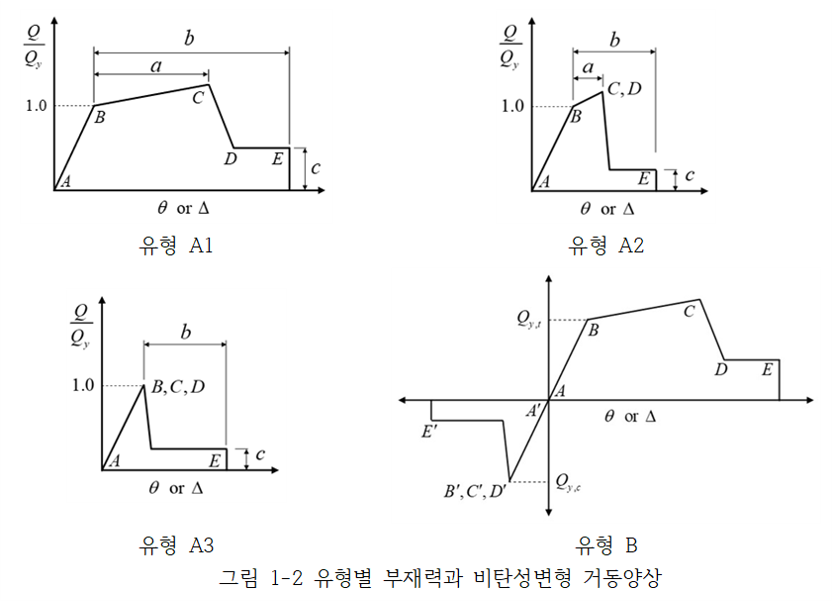
\includegraphics[width=0.99\textwidth]{image1-2}
		\end{figure}

	\end{frame}


	\begin{frame}
		\begin{figure}
			\centering
			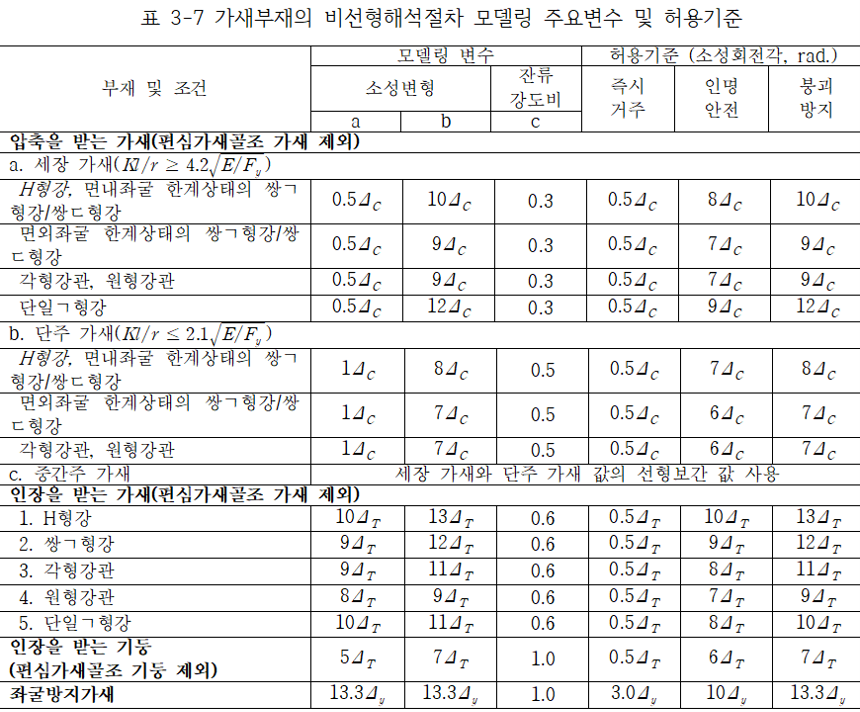
\includegraphics[width=.99\textwidth]{table3-7}
		\end{figure}
	\end{frame}



	\begin{frame}{3.5 가새}

	\textbf{3.5.2 가새의 강성}
	
	3.5.2.3 비선형동적절차
	
	\begin{enumerate}
		\item[(1)] 비선형동적절차의 이력거동 모델링은 실험이나 정밀해석을 통해 얻어진 관계를 사용할 수 있다. 
		\item[(2)] 가새 부재의 거동에 관한 실험자료가 없는 경우 3.5.2.2절에 제시된 부재의 일반화된 부재력--변형 모델을 가새의 역량경계(capacity boundary) 또는 포락곡선을 정의하는데 사용할 수 있다. 
		\item[(3)] 반복하중에 대한 가새의 이력거동이 모델링에 포함되어야 하며, 다음의 사항을 따른다. 
		\begin{enumerate}[label=\large\protect\textcircled{\small\arabic*}]
			\item 반복이력하중과 변형경로는 역량경계 또는 포락곡선을 넘어선 범위에서 교차하지 않아야 한다.  
			\item 서로 다른 요소의 명확한 반복저감 기울기가 상이할 경우, 반복재하 및 제하에 따른 강성저감, 강도저감이나 in-cycle strength degradation을 포함한 반복이력특성을 모델링해야 하며, 실제 거동에 근접하도록 모델링 하여야 한다. 
		\end{enumerate}
	\end{enumerate}
	\end{frame}
	
	



	\begin{frame}{3.5 가새}

	\textbf{3.5.3 가새의 강도}
	
	3.5.3.1 선형동적절차
	
	\begin{enumerate}
		\item[(1)] 변형지배거동인 가새 부재의 예상부재강도 $Q_{CE}$는 다음과 같이 산정한다. 
		\begin{enumerate}[label=\large\protect\textcircled{\small\arabic*}]
			\item 압축력을 받는 가새의 예상부재강도 $Q_{CE}$는 가새의 전체좌굴 또는 국부좌굴 한계상태 강도 중 최솟값으로 한다.  
			\item 압축력을 받는 가새의 예상압축강도 $P_{CE}$는 $\ulcorner$건축물 강구조 설계기준$\lrcorner$에 따라 산정하며 항복강도는 예상재료강도 $F_{ye}$를 사용한다. 대각가새가 중앙에서 교차하고 일반적인 거셋플레이트를 사용하는 일반 X형 가새의 경우, 각 가새의 유효길이는 양방향 좌굴축에 대한 거셋플레이트를 제외한 가새길이에 0.5배한 값을 사용한다.
			\item V형, 역V형 및 단일가새의 경우, 거셋플레이트를 사용하지 않을 시 가새의 유효길이는 가새 양쪽 단부 사이의 거리를 사용하고, 가새를 강접합할 경우에는 작용점 사이 거리에 0.7배한 값을 사용한다. 
			\item 인장력을 받는 가새의 예상부재강도 $Q_{CE}$는 3.2절 기둥의 기준을 따른다. 
		\end{enumerate}		
	\end{enumerate}
	\end{frame}	


	\begin{frame}{3.5 가새}

	\textbf{3.5.3 가새의 강도}
	
	3.5.3.1 선형동적절차
	
	\begin{enumerate}
		\item[(2)] 힘지배거동인 가새 부재의 하한부재강도 $Q_{CL}$은 3.2절 기둥의 기준을 따른다. 
\begin{block}{ASCE 41-17 9.5.2.4 AC for CBF}
Beams, their connections, and supporting members in V-type or inverted V-type braced frames shall be evaluated as force-controlled actions to resist the unbalanced load effects (...).  
	\end{block}	
	\begin{block}{ASCE 41-17 9.5.3.4 AC for EBF}
Shear and flexure in link beams shall be considered deformation-controlled actions. All other actions, and actions on other EBF somponents, shall be considred force controlled. 
	\end{block}	
	\begin{block}{AISC 342-XX (Draft): STRUCTURAL STEEL BRACED BRAME}
		$m=1$ when the beam is classified as a slender section (...) and the top flange is laterally braced at a spacing exceeding limiting laterally braced length for the limit state of inelastic LTB.
	\end{block}	
	\end{enumerate}
	\end{frame}	
	
	\begin{frame}{3.5 가새}

	\textbf{3.5.3 가새의 강도}
	
	3.5.3.2 비선형정적 및 동적절차
	
	\begin{enumerate}
		\item[(1)] 비선형정적절차의 경우 표 3-7에 따라 그림 1-2과 같은 비선형 부재력--변형 관계를 결정한다. 가새의 예상부재강도 $Q_{CE}$는 선형절차와 동일한 값을 사용한다. 
		\item[(2)] 비선형동적절차의 이력거동 모델링은 실험이나 정밀해석을 통해 얻어진 관계를 사용할 수 있으며, 포락곡선으로는 표 3-7에 사용된 모델을 적용할 수 있다. 
	\end{enumerate}
	\end{frame}	


	\begin{frame}
		\begin{figure}
			\centering
			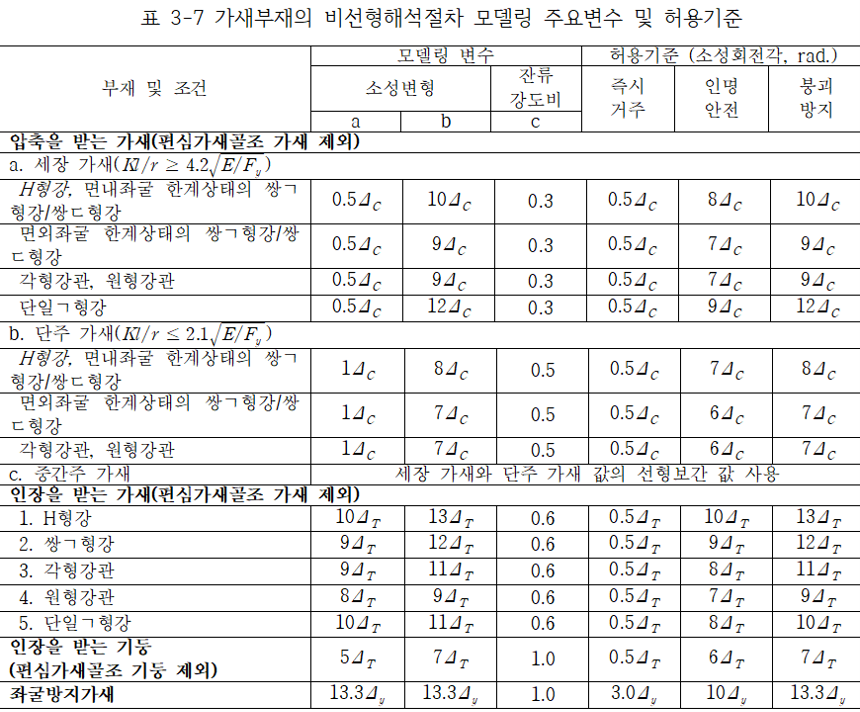
\includegraphics[width=.99\textwidth]{table3-7}
		\end{figure}
	\end{frame}
		

	\begin{frame}{3.5 가새}

	\textbf{3.5.4 가새의 허용기준}
	
	3.2.4.1 일반사항
	
	\begin{enumerate}
		\item[(1)] 중심가새골조의 가새 부재는 변형지배거동으로 분류한다. 
		\item[(2)] 편심가새골조의 가새 부재는 힘지배거동으로 분류한다. 
		\item[(3)] 거셋플레이트, 볼트, 용접 및 기타 접합요소를 포함한 가새접합부에 작용하는 압축, 인장, 전단 및 휨은 힘지배거동으로 분류한다. 	
	\end{enumerate}		
	
	3.2.4.2	선형동적절차
	
	\begin{enumerate}
		\item[(1)] 중심가새의 $m$계수는 표 3-8을 따른다. 
		\item[(2)] V형 또는 역V형 가새골조 내 보와 보의 접합부 및 지지부재는 중력하중과 불균형하중 효과에 저항하기 위해 힘지배거동으로 평가하여야 한다. 
		\item[(3)] 불균형하중 효과는 인장력을 받는 가새의 예상항복강도와 압축력을 받는 가새 예상압축강도의 30\%를 사용하여 산정한다. 
	\end{enumerate}
	
	3.2.4.3 비선형 정적 및 동적절차: 가새 부재의 변형한계는 표 3-2, 3-6 및 3-7을 사용한다.  
	\end{frame}	


	\begin{frame}
		\begin{figure}
			\centering
			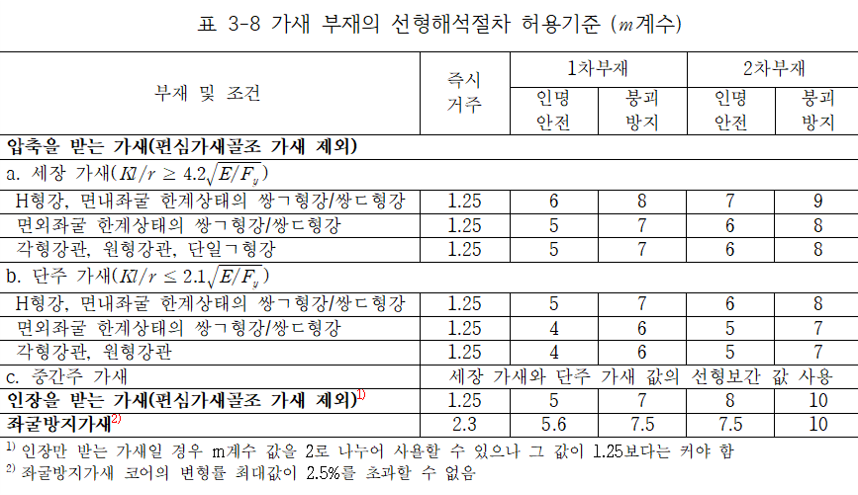
\includegraphics[width=.99\textwidth]{table3-8}
		\end{figure}
	\end{frame}
		